\documentclass[a4paper,10pt]{article}

\usepackage[margin=3cm]{geometry}
\usepackage[pdftex]{graphicx}
\usepackage{verbatim,url}

\begin{document}

\title{
  {\normalsize
    Introduction to Algorithms, Data Structures, and Problem Solving\\
    DA4002 (HT11) Halmstad University}\\
  Assignment for Project 1: Complexity Analysis\\
}
\author{
  \texttt{roland.philippsen@hh.se}
}
\maketitle



\section{Introduction}

An important aspect of the ITADS course is to teach participants how to evaluate possible solutions for a given problem.
Complexity analysis is a tool within this evaluation process.
The lecture and the course book discuss several theoretical aspects of computational complexity, with a focus on how runtime grows with problem size.
The first project complements the theoretical treatment with hands-on experience.
It provides a practical and empirical understanding of the theory, and prepares the participants to make informed choices in real-life programming situations.

The deadline for handing in the source code and the report is \textbf{Friday, September 30, 2011, at 18h00}.
Teams who miss the deadline will receive a penalty by lowering their grade by one.
In case of exonerating circumstances, such as sickness certified by a medical doctor, a deadline extension will be granted.
Participants must notify the lecturer of such circumstances as soon as possible when they arise.



\section{Assignment}

Participants are provided with a collection of classes and two fully functional example applications.
The first is a benchmark for container operations, the second is a benchmark for sorting algorithms.
All code can be compiled with the help of the command ``\texttt{make}'' which relies on the provided \texttt{Makefile}.



\subsection{Overview}

Each team first chooses one of the two provided examples as starting point.
This means you will either investigate the time complexity of container operations (Alternative A), or the complexity of sorting algorithms (Alternative B).
The first set of mandatory tasks for each alternative will be to extend the provided code with additional implementations.
The remaining ``bonus'' tasks will be to make the benchmark more complete, and there are several possible ways of achieving this.
For example, add different types of input data, compare theoretical with practical complexity, or make the measurements more statistically meaningful.
More details about the mandatory task will be provided in sections~\ref{sec:task1a} and~\ref{sec:task1b}.
Possible avenues for the bonus tasks are discussed in section~\ref{sec:tasks2}.

Keep in mind that writing the report is an integral part of the project, so do not spend too much time on extending the functionality.
Well-performed mandatory tasks that are properly documented in the report will receive a good grade.
In order to achieve an excellent grade, at least one bonus task needs to be done.

It is important to note that teams are expected to manage their resources by themselves.
This includes apportioning the time available for finding information online and in the book, developing and debugging code, running the benchmarks, and documenting the work.
How these aspects are shared between the team members is for each team to decide.



\section{Container Operation Benchmark}

\begin{figure}
  \centering
  \fbox{
    \begin{minipage}{0.8\columnwidth}
      \footnotesize
      \verbatiminput{console-ExampleA.txt}
  \end{minipage}}
  \caption{
    Typical console output from \texttt{ExampleA}.
    The table with the running times gives feedback while the benchmark is being run.
    The list of commands at the end allows to view and create figures.
  }\label{fig:exa-console}
\end{figure}
  
\begin{figure}
  \centering
  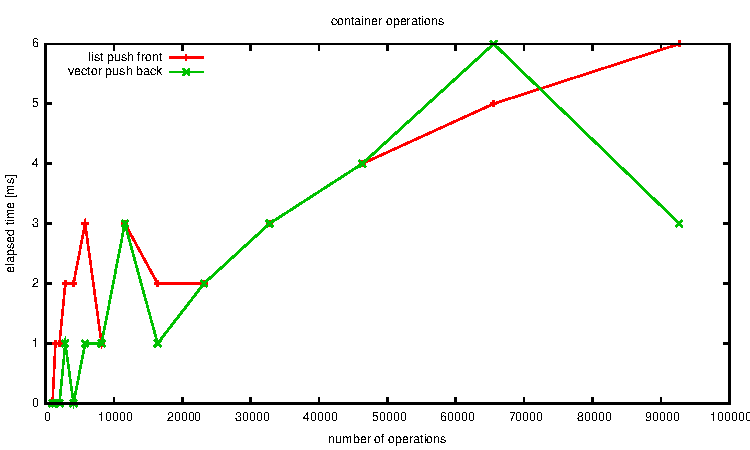
\includegraphics[width=0.8\columnwidth]{plot-ExampleA.pdf}
  \caption{
    Execution time plot produced by running example A.
  }\label{fig:exa-plot}
\end{figure}

The aim of this benchmark is to determine how long it takes to perform fundamental container operations, such as insertion and removal of elements.
The provided application is in \texttt{ExampleA.java}.
It is limited to two container implementations (doubly-linked lists and dynamically expanding arrays).
It is also limited to just a single container operation (repeated insertion at the front or back of the container).

Example A is launched by the command ``\texttt{java ExampleA}.''
It produces console output similar to the one shown in figure~\ref{fig:exa-console}.
Note that the application relies on reusable code for logging execution times, saving these logs to a file, and producing figures from the data.
Figure~\ref{fig:exa-plot} was produced by running the automatically generated ``\texttt{gnuplot log-1316350931155-all-pdf.plot}'' command.
Note that the name of the files containing the data log and the plot scripts changes each time that \texttt{ExampleA} is run (see section~\ref{sec:remarks} for more details).



\subsection{Mandatory Tasks for Alternative A}\label{sec:task1a}

First, implement a binary search tree which stores strings, and measure how long it takes to insert $N$ random strings into it.
You can use the code of \texttt{Dictionary.java} provided in exercise 3.3 as a starting point, but beware that for this project we only store a value, instead of a key-value pair.
Verify that your tree functions correctly, and produce benchmark plots that clearly illustrate the different growth rates of item insertion for trees when compared to sequence containers.

Then, extend the benchmark to also measure the time it takes to remove $N$ items from each container.
Choose fast operations, such as \texttt{popBack} for the list and the vector, and \texttt{removeMin} for the binary search tree.
First insert $N$ items without measuring that time, and then measure the time required to remove all items one by one.
Produce a benchmark plot which clearly illustrates the differences between the remove operation based on container type.



\section{Sorting Algorithm Benchmark}

\begin{figure}
  \centering
  \fbox{
    \begin{minipage}{0.8\columnwidth}
      \footnotesize
      \verbatiminput{console-ExampleB.txt}
  \end{minipage}}
  \caption{
    Typical console output from \texttt{ExampleB}.
    Similarly to figure~\ref{fig:exa-console}, the table is produced while the benchmark is being run.
    Again, the list of commands at the end allows to view and create figures.
  }\label{fig:exb-console}
\end{figure}

\begin{figure}
  \centering
  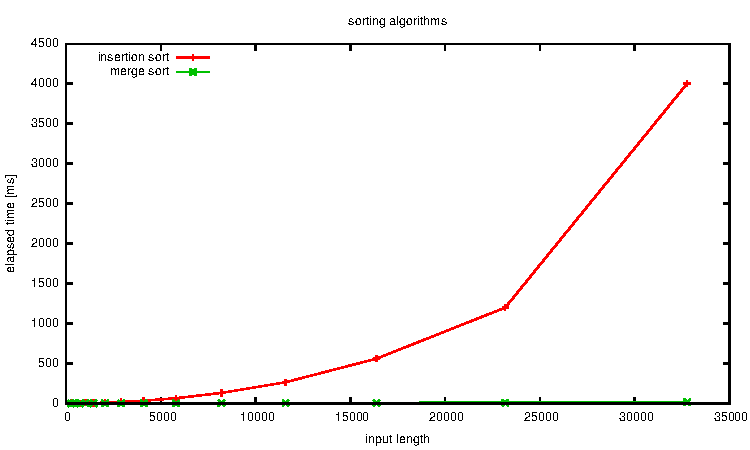
\includegraphics[width=0.8\columnwidth]{plot-ExampleB-all.pdf}\\
  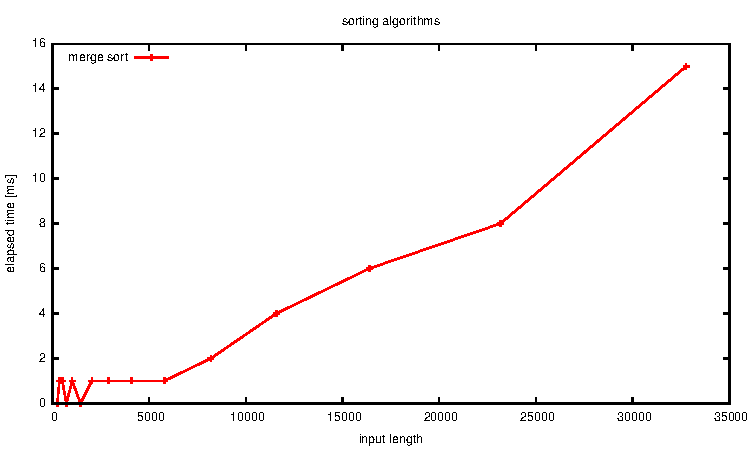
\includegraphics[width=0.8\columnwidth]{plot-ExampleB-zoom.pdf}
  \caption{
    Execution time plot produced by running example B.
    The bottom figure is a zoom on the running time of merge sort.
  }\label{fig:exb-plot}
\end{figure}

The aim is to determine how long it takes to sort sequences of varying lengths.
The provided application is in \texttt{ExampleB.java}.
It is limited to two search algorithms (insertion sort and merge sort).
It is also limited to just a single class of input data (arrays of random strings).

Example B is launched by running ``\texttt{java ExampleB}.''
It produces console output like the one in figure~\ref{fig:exb-console}.
It relies on the same logging and plotting functionality as example A.
Figure~\ref{fig:exb-plot} shows two figures based on this run, produced with the two PDF plot scripts mentioned in the console output.



\subsection{Mandatory Tasks for Alternative B}\label{sec:task1b}

\begin{table}
  \centering
  \begin{tabular}{l|l|l}
    \textbf{algorithm} & \textbf{difficulty} & \textbf{link} \\
    \hline
    cocktail sort    & easy         & \url{http://en.wikipedia.org/wiki/Cocktail_sort} \\
    selection sort   & easy         & \url{http://en.wikipedia.org/wiki/Selection_sort} \\
    gnome sort       & easy         & \url{http://en.wikipedia.org/wiki/Gnome_sort} \\
    shell sort       & intermediate & \url{http://en.wikipedia.org/wiki/Shell_sort} \\
    comb sort        & intermediate & \url{http://en.wikipedia.org/wiki/Comb_sort} \\
    cycle sort       & intermediate & \url{http://en.wikipedia.org/wiki/Cycle_sort} \\
    quicksort        & hard         & \url{http://en.wikipedia.org/wiki/Quicksort} \\
    heapsort         & hard         & \url{http://en.wikipedia.org/wiki/Heapsort} \\

    %Binary tree sort & easy\footnote{When using an existing binary tree implementation, such as the one from the Java Collections library.}
    %                          & \url{http://en.wikipedia.org/wiki/Binary_tree_sort} \\
    %Strand sort      & medium\footnote{When using a full-featured list implementation, e.g.\ from the Java Collections library.
    %                                   The provided \texttt{StringList} class would first need to be extended somewhat. }
    %                          & \url{http://en.wikipedia.org/wiki/Strand_sort} \\
  \end{tabular}
  \caption{
    List of sorting algorithms which can be implemented as part of alternative B.
  }\label{tab:sorting-algorithms}
\end{table}

Table~\ref{tab:sorting-algorithms} list some sorting algorithms which can added to the benchmark.
The list excludes bubble sort, insertion sort, and merge sort, because they are either provided as part of the project starting point or have been treated during an exercise.
The (estimated) difficulty of implementing each algorithm is also given, along with a link to a Wikipedia page providing more details.

The mandatory tasks of alternative B are:
First, add algorithms from table~\ref{tab:sorting-algorithms} to the sorting benchmark.
Each team should choose either \textbf{two \emph{easy}} algorithms, or \textbf{one \emph{intermediate}} algorithm.
Then, extend the sorting benchmark to also measure the time it takes each algorithm to sort data which is already sorted, as well as data which is sorted in reverse.
Create clear plots which illustrate the differences between the sorting algorithms in all three cases of input data (random, sorted, and reversed).



\section{Bonus Tasks}\label{sec:tasks2}

Choose \textbf{one} of the following bonus tasks in order to achieve an excellent grade.
You are of course free to perform more than one bonus task, but keep in mind that documenting your choice and its results will also take some time.
The first list of bonus tasks is applicable to either the container or the sorting benchmark.
The following two lists are specific to each alternative.

\begin{itemize}

\item
  Make the data containers or sorting algorithms generic.
  Then create a benchmark which determines whether there is a significant performance difference between data of type \texttt{String} or \texttt{Integer}.
  You will need to extend the \texttt{Factory} with a method to create arrays of random integers, similar to the one which creates random strings.
  Create plots which clearly demonstrate your results.
  
\item
  Determine how well the running times match the typical complexity classes.
  This is done by computing the theoretical growth rate according to the $F(N)$ of the $O(F(N))$ expression, dividing the actual runtime by it, and detecting whether that ratio converges to a non-zero value.
  You will notice that the running time measurements can be quite ``noisy.''
  Create corresponding plots and discuss your findings in the report.
  
\item
  Reduce the effect of ``noise'' in the runtime measurements by performing each measurement several times and taking the average.
  The \texttt{LogSeries} class, which is used to log the actual runtimes, provides 4 methods to help with this task.
  Find those methods, read their documentation, and apply them to the benchmark.
  Create plots which compare the data with and without averaging, and discuss your findings.
  
\end{itemize}


\subsection*{For Alternative A}

\begin{itemize}

\item
  Investigate if and how the running times depend on the order of the input data.
  Create benchmarks for inserting already-sorted data, data which is sorted in reverse, and data which has many duplicate items.
  Produce benchmark plots that clearly demonstrate the different running times, and dicsuss the measured effects.

\item
  Compare the running times for finding strings, using the \texttt{find} methods of \texttt{StringList} and your search tree implementation.
  The \texttt{Factory} provides a method which makes it easy to generate a list of strings to find:
  ``\texttt{Factory.create\-Samples(data, 1000, 0.1);}'' will create an array with 1000 strings, where 90\% are taken from the provided \texttt{data}, and the remaining 10\% are randomly generated.
  Verify that your \texttt{find} method works, and produce benchmark plots that clearly demonstrate the different running times of finding items in lists and trees.

\item
  Add a hash table and a balanced binary tree from the Java Collections library to the benchmark.
  Use \texttt{java.util.HashSet<String>} and \texttt{java.util.TreeSet<String>}.
  Produce benchmark plots that clearly demonstrate the different running times, and dicsuss the measured effects.

\end{itemize}



\subsection*{For Alternative B}

\begin{itemize}

\item
  Add two \emph{intermediate} algorithms from table~\ref{tab:sorting-algorithms} to the benchmark.

\item
  Add one \emph{hard} algorithm from table~\ref{tab:sorting-algorithms} to the benchmark.
  
\end{itemize}



\section{Additional Remarks}\label{sec:remarks}



\subsection{Managing the Automatically Generated Files}

The provided code for logging and and producing figures has a tendency to clutter the working directory with many files.
The idea is to never delete data or plots, unless explicitly desired by the user.
In order to simplify the management of these files, they follow very strict naming conventions.

\begin{description}
\item[prefix:]
  all automatically produced files begin with \texttt{log-}
\item[timestamp:]
  number which changes each time the application is run, for example \texttt{1316351173681}
\item[optional annotations:]
  short dash-separated tokens such as \texttt{all-scr} which are used to separate different types of plots from each other
\item[extension:]
  \texttt{.data} denotes a text file with logged data, \texttt{.plot} is a plot script which reads the corresponding data file to produce a figure (either on screen or as a PDF), and \texttt{.pdf} is a figure produced by the corresponding script file.
\end{description}

It is recommended that the ``good'' data, plot scripts, and the produced figures are manually copied to a separate directory in order to save them.
Also, it is a good idea to rename them in the process, for example to indicate what is on the plot.
Then, it will be much easier to include the data and plots in the report.

For example, suppose that \texttt{log-1316351173681.data} contains the data of a benchmark run which was particularly good at showing some effect.
Then, the following sequence of \textsc{Unix} commands will save the data and the associated plots in a separate directory with a more descriptive name:

\begin{verbatim}
gnuplot log-1316351173681-all-pdf.plot
gnuplot log-1316351173681-sep-pdf.plot
mkdir good-example-directory-name
mv log-1316351173681* good-example-directory-name/.
\end{verbatim}

Of course, adapt the directory name to something more meaningful first.
Then, it will be possible to remove most (or even all) of the other \texttt{log-} files to make the project directory more tidy.



\subsection{Customizing the Plot Scripts}

The automatically generated scripts for plotting the data logs are text files with \texttt{gnuplot} commands.
It is possible to edit these scripts in order to customize the plots.
It is also possible to run \texttt{gnuplot} in interactive mode, and copy-paste-adapt individual commands from the script files.
To enter interactive mode, simply launch \texttt{gnuplot} without arguments.

Gnuplot comes with extensive online documentation~\cite{gnuplot}, and it has a built-in \texttt{help} command, too.



\subsubsection{Example: Creating PNG Figures}

Depending on the software used to prepare the project report, it may be better to produce figures in PNG format rather than the PDF format provided by the automatically generated scripts.
This is easy to achieve by changing the corresponding \texttt{log-*-pdf.plot} script:

\begin{enumerate}
\item
  open the script in a text editor
\item
  change the \texttt{term} variable to \texttt{png} instead of \texttt{pdf} (this is on or near line 5)
\item
  change the \texttt{output} filename to something ending in \texttt{.png} instead of \texttt{.pdf} (this is on or near line 6)
\item
  safe the modified script and run it using ``\texttt{gnuplot modified-script-filename}'' (of course, change the filename to whatever you saved the file as)
\end{enumerate}



\subsubsection{Example: Merging Parts from Different Plots}

Suppose there are two log files \texttt{log-123.data} and \texttt{log-456.data} and their corresponding plot scripts.
You wish to create a figure with the first data set from \texttt{log-123.data} and the second data set from \texttt{log-456.data}.

\begin{enumerate}
\item
  choose one of the plot files as starting point and copy it to a new file, for example:\\
  \texttt{cp log-123-all-scr.plot log-fused.plot}
\item
  open \texttt{log-fused.plot} in a text editor and remove the parts you do not want to plot anymore
\item
  copy-paste the relevant plot commands from the other script (\texttt{log-456-all-scr.plot} in this example)
\item
  safe \texttt{log-fused.plot} and run it using ``\texttt{gnuplot log-fused.plot}''
\end{enumerate}

Note that the \texttt{plot} command creates a fresh plot, if you want to have several data sets on the same plot they must come as comma-separated entries on one line.



\footnotesize
\bibliographystyle{plain}
\bibliography{itads-bibliography}

\end{document}
